\documentclass{beamer}
\usetheme{CambridgeUS}
\title{Foot classifier}
\subtitle{Progetto IC}
\author{Luigi Lomasto, Marco Mecchia}
\date{29 Febbraio 2016}
\usepackage[italian]{babel}
\usepackage[latin1]{inputenc}
\usepackage[T1]{fontenc}
\usepackage{graphicx}
\usepackage{pgf}
\usepackage{multimedia}
\usepackage{listings}
\usepackage{amsmath}

\begin{document}
	\begin{frame}
		\maketitle
		Prof. Roberto Tagliaferri \newline
		Dott. Paola Galdi \newline
		Dott. Angela Serra
	\end{frame}
	
\begin{frame}
	\frametitle{Outline}
	\tableofcontents
\end{frame}

\section{Introduzione al problema}

\begin{frame}
	\frametitle{Definizione}
    Il lavoro svolto ha avuto come obiettivo quello di addestrare un'classificatore in modo da classificare successivamente i piedi in base alle seguenti patologie: 
	\newline
	 \begin{itemize}
	\item Cavo
	\item Piatto
	\item Normale
	\item Valgo
    \end{itemize}
\end{frame}

\begin{frame}
	\frametitle{Patologie}
	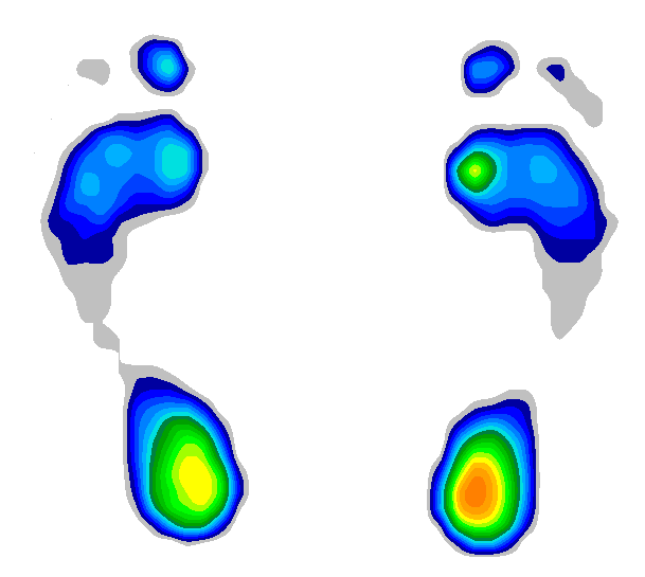
\includegraphics[keepaspectratio,height=95px]{immagini/0_cleared.png}
	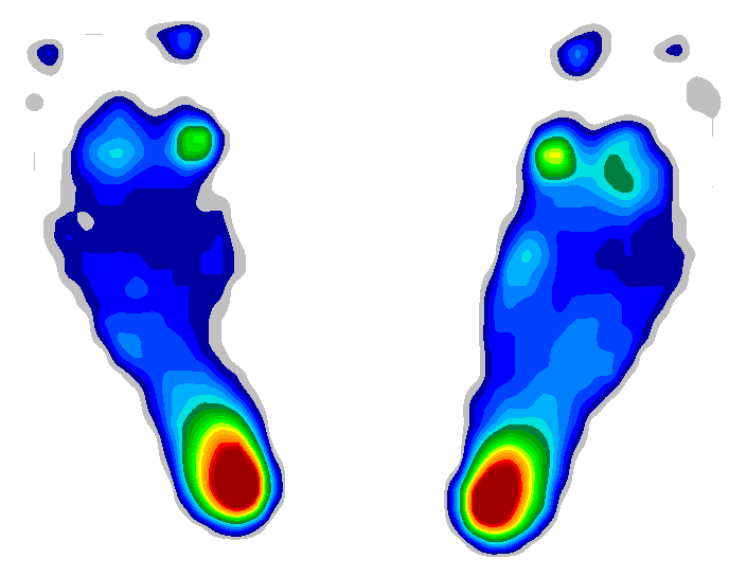
\includegraphics[keepaspectratio,height=95px]{immagini/1_cleared.png}
	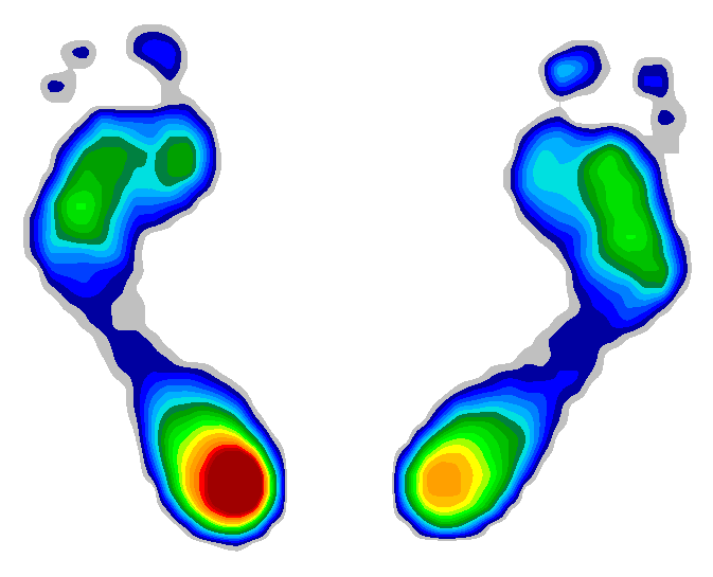
\includegraphics[keepaspectratio,height=95px]{immagini/2_cleared.png}
\end{frame}

\section{Dataset}
\begin{frame}
	\frametitle{Struttura del dataset}
	Il dataset � costituito da 190 piedi (95 coppie) di cui:
	\begin{itemize}
		\item 121 Cavi
		\item 13 Piatti
		\item 56 Normali
	\end{itemize}
	per la prima classe di patologie, mentre:
	\begin{itemize}
		\item 88 Valghi
		\item 102 Normali
	\end{itemize}
	per la seconda classe di patologie. In quest'utlima non sono presenti piedi vari.
\end{frame}
\section{Preprocessing del dataset}
\begin{frame}
	\frametitle{Preprocessing dei dati}
	Prima di estrarre le features � stata necessaria una fase di preprocessing per memorizzare le immagini in matrici. Di seguito sono elencate le fasi di lavoro svolte per il preprocessing.
	\begin{itemize}
		\item Conversione delle immagini .bmp in .png.
		\item Pulizia delle immagini (rimozione del baricentro).
		\item Trasformazione delle immagini in scala di grigio.
		\item Rotazione e ritaglio dei piedi.
	\end{itemize}
	\centering
	 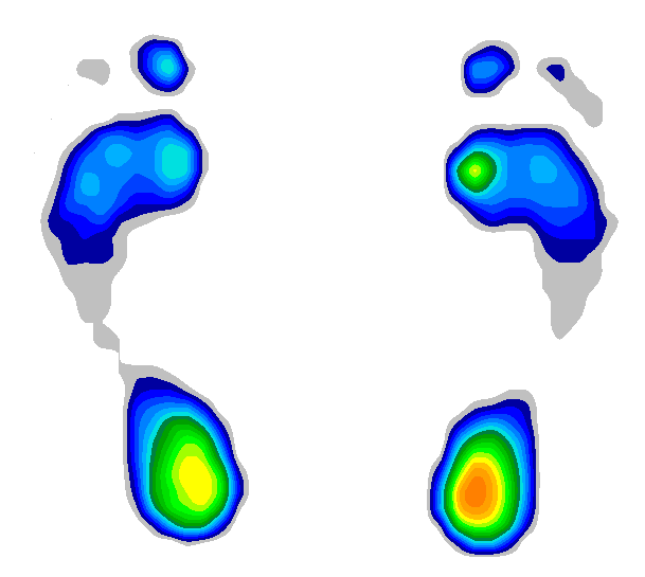
\includegraphics[keepaspectratio,height=80px]{immagini/0_cleared.png} 
	 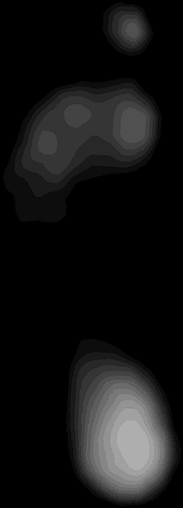
\includegraphics[keepaspectratio,height=80px]{immagini/sin.png}
	 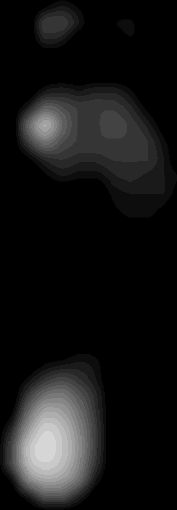
\includegraphics[keepaspectratio,height=80px]{immagini/des.png}
\end{frame}

\section{Features extraction}
\begin{frame}
	\frametitle{Features extraction}
	Terminata la fase di preprocessing siamo passati alla fase di features exstraction. Nel nostro caso, le regioni d'interesse di ogni piede differiscono significativamente tra loro. Per questo motivo, � stato necessario implementare algoritmi ad-hoc per l'estrazione delle features. 
	\newline
	Dovendo lavorare con due classi di patologie:
	\begin{itemize} 
		\item Cavo, piatto e normale.
		\item Valgo e normale.
    \end{itemize} 
   
   sono stati implementati due algoritmi per l'estrazione delle features.
\end{frame}

\subsection{Features primo classificatore}
\begin{frame}
	\frametitle{Features primo classificatore (1/2)}
	Le features estratte per le patologie appartenenti alla prima classe sono le seguenti:
	\begin{itemize}
		\item \textbf{lengthMinIstmo:} esprime la lunghezza minima che assume l'istmo.
		\item \textbf{lengthMediaIstmo:} esprime la lunghezza media dell'istmo.
		\item \textbf{lengthMaxAvampiede:} esprime la massima lunghezza che assume l'avampiede.
		\item \textbf{indexPathology:} Si ottiene dal rapporto $\frac{lengthMaxAvampiede}{lengthMinIstmo}$
		\item \textbf{mediumPressure:} Indica la pressione media esercitata dal piede.
	\end{itemize}
	
\end{frame}
\begin{frame}
	\frametitle{Features primo classificatore (2/2)}
    \centering
     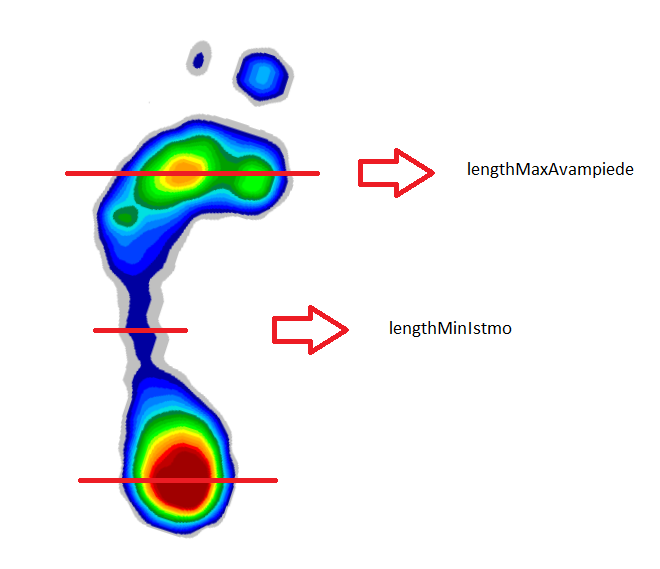
\includegraphics[keepaspectratio,height=220px]{immagini/Immagine.png}
\end{frame}

\subsection{Features secondo classificatore}
\begin{frame}
	\frametitle{Features primo classificatore (1/2)}
	Le features estratte per le patologie appartenenti alla seconda classe sono le seguenti:
	\begin{itemize}
		\item  \textbf{diffPosition:} indica la distanza tra il centro del tallone e il centro della zona di massima pressione.
		\item  \textbf{approssimated:} Simile alla varaibile precedente. Varia per due motivi: si considera in valore assoluto ed assume valore pari a 0 se la differenza � inferiore a 10 (pixel). 
		
		distanceBoundLeft,distanceBoundRight
	\end{itemize}
	
\end{frame}
\begin{frame}
	\frametitle{Features primo classificatore (2/2)}
	\centering
	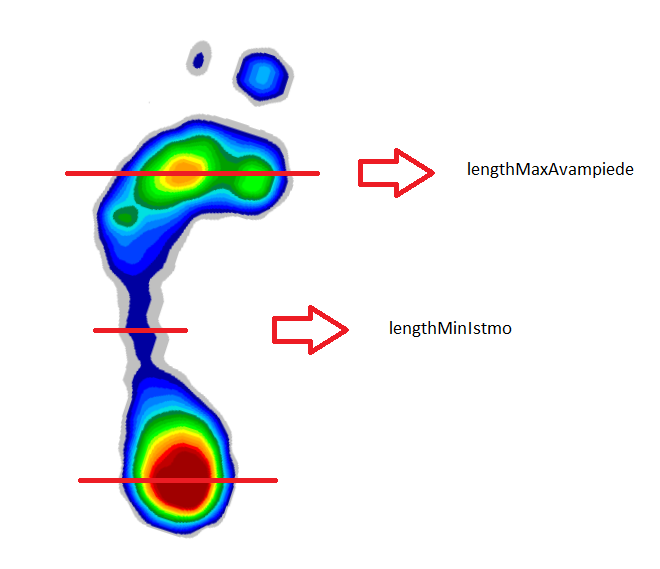
\includegraphics[keepaspectratio,height=220px]{immagini/Immagine.png}
	
\end{frame}

\section{Scelta dei classificatori}
\section{Risultati}
\section{Conclusioni}

\end{document}
